\chapter{Model-based receding horizon control}
\label{chap:rhc}
\chaptermark{Model-based receding horizon control}

In this chapter, we address the power tracking problem of secondary frequency regulation using a model-based receding horizon control method~\cite{Rawlings2009a}.  Previous work has used a high-fidelity numerical simulation as a state-space representation of the wind farm for the associated optimal control problem~\cite{Goit2015a}. Instead, we use the time-varying one-dimensional PDE wake model discussed in Section~\ref{sec:dynwake-1d}. Feedback from measurements of wind velocity at each turbine is used to correct modeling errors at each control step. By reducing the number of states by many orders of magnitude, the online optimization problem can be solved in real time. We test the controller on a LES wind farm test system ith actuator disk turbine models, discussed in more detail in Section~\ref{subsec:methods-les-farm}. A diagram of the controlled wind farm system is shown in Figure~\ref{fig:diagram}.

\begin{figure}[]
\centering
\includegraphics[width=\textwidth]{./fig/block_diagram.pdf}
\caption{Diagram of the controlled wind farm system used to track a power reference signal $\text{P}_\text{ref}$. The model-based receding horizon controller (left block) sends local thrust coefficient control signals $\text{C}_\text{T}'$ to the wind farm test system (right block) and closed-loop feedback is based on wind speed measurements $\mathbf{u}$ at each turbine that are passed though an error correction filter. The wind farm is depicted via instantaneous streamwise velocity contours from LES, where slow velocity is blue and high velocity is red. Turbine locations are shown as black lines toward the end of the domain.}
\label{fig:diagram}
\end{figure}

\section{Control design}
\label{sec:rhc-control}

We now incorporate the model developed in Section~\ref{sec:dynwake-1d} into a model-based receding horizon control framework~\cite{Rawlings2009a}. This approach to the power-tracking problem iteratively solves a finite-time optimal control problem, as shown in the schematic diagram of Figure~\ref{fig:receding_horizon}. At each iteration, the problem is solved for a time horizon of length $T$. The controls computed for each iteration, however, are only implemented for a time period of length $T_A < T$, after which the optimal control problem is re-solved~\cite{Bewley2001a, Goit2015a}. Closed-loop error correction is provided using the temporally-damped correction of Section~\ref{sec:estimation-damped}.

The local thrust coefficient $C_T'$ is used as the control variable in the receding horizon control. While generator torque or blade pitch angle are more realistic wind turbine control variables~\cite{Pao2011a}, the local thrust coefficient can parameterize these controls~\cite{Goit2015a}. The local thrust coefficient, however, should be limited to ensure realistic operating conditions. For ease of implementation, we add a regularization term to the cost functional of the optimal control problem described below instead of constraining the optimal control problem using box constraints~\cite{Goit2015a}. 

For each optimization iteration, the power tracking problem can be rewritten as a minimization problem of a cost functional $\mathcal{J}$ constrained by the wake model
\begin{align}
\label{eq:minimize_J}
\underset{\mathbf{C_{T}'}, \mathbf{q}}{\text{minimize}} \qquad & \mathcal{J}(\mathbf{C_T'}, \mathbf{q} ) \\
\label{eq:constraint1}
\text{subject to} \qquad & \frac{\partial \delta u_n}{\partial t} +U_\infty \frac{\partial \delta u_n}{\partial x} = -w_n(x) \delta u_n(x,t) + f_n(x,t) \\
\label{eq:constraint2}
& \hat{u}_n (t) = U_\infty - \int_0^L  \left(\sum_{m=1}^N \delta u_m^2(x,t)\right)^{1/2}G(x - s_n) \, dx + \epsilon_n(t),
\end{align}
where the states are $\mathbf{q} \equiv [\boldsymbol \delta \mathbf{u}(x,t), \mathbf{\hat{u}}(t)]$. We use a cost functional
\begin{equation}
\begin{split}
\mathcal{J} =& \frac{1}{\mathcal{P}^2T}\int_0^T \left( \sum_{n=1}^{N}\hat{P}_n(t)  - P_\text{ref}(t)  \right)^2 \, dt + \frac{\eta}{T}\sum_{n=1}^{N} \int_0^T \left( C_{Tn}'(t)  - C'_{T\text{ref}}\right)^2 \, dt \\
&+ \gamma T\sum_{n=1}^{N} \int_0^T \left( \frac{d C_{Tn}'}{dt}\right)^2 \, dt
\end{split}
\end{equation}
that is the weighted sum of three terms: the first describes the reference tracking goal; the second penalizes deviations away from the pre-control thrust coefficient $C'_{T\text{ref}}$,  which can be seen as a relaxation of bounds on the local thrust coefficient; and the third penalizes large time derivatives of the thrust coefficients to prevent high frequency oscillations in the control. The constant $\mathcal{P} = M \frac{1}{2}\rho\frac{ \pi D^2}{4} U_\infty^3 $ normalizes the power of each row of $M$ turbines and makes the regularization cost functionals the same order of magnitude as the tracking cost functional. The weighting coefficients $\eta$ and $\gamma$, which are much smaller than one, are the relative weights of the regularizations.

\begin{figure}[t]
\centering
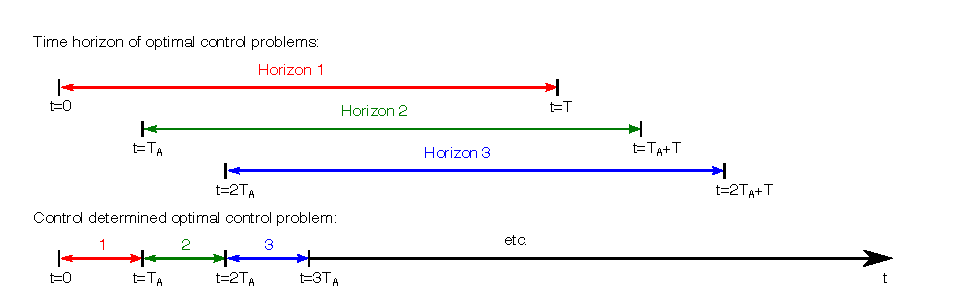
\includegraphics[width=\textwidth]{./fig/receding_horizon.pdf}
\caption{Schematic diagram of the receding horizon control approach.}
\label{fig:receding_horizon}
\end{figure}

We solve the optimization problem by reformulating it using the unconstrained reduced cost functional $\tilde{\mathcal{J}}(\mathbf{C_T'}) = \mathcal{J}(\mathbf{q},\mathbf{C_T'})$~\cite{Bewley2001a, Goit2015a} and minimizing this modified problem in the manner discussed in Section~\ref{sec:methods-pdeopt}. The minimization is performed for a fixed number of iterations using the gradient-based nonlinear Polak-Ribi\`{e}re conjugate gradient method~\cite{Press2007a} combined with the Mor\'{e}-Thuente line search method~\cite{More1994a}. Each Polak-Ribi\`{e}re conjugate gradient iteration requires the computation of the gradient of the reduced cost functional $\nabla\tilde{\mathcal{J}}$ for a given control $\mathbf{C_T'}(t)$. Even for this simplified wake model, direct finite differencing is impractical; instead the gradient is computed using one backward simulation of the adjoint equations, as discussed in Section~\ref{sec:methods-pdeopt}.

The gradient of the reduced cost functional and the adjoint equations are derived using the formal Lagrangian method~\cite{Goit2015a, Borzi2011a}. A Lagrangian is constructed with adjoint variables $\mathbf{q^*} \equiv [\boldsymbol \delta \mathbf{u}^*(x,t), \mathbf{\hat{u}^*}(t)]$ as Lagrange multipliers, which are denoted by stars
\begin{align}
&\mathcal{L}(\mathbf{C_T'}, \mathbf{q}, \mathbf{q^*}) = \mathcal{J}(\mathbf{C_T'},\mathbf{q}) \\
&+ \sum_{n=1}^N \int_0^T \int_0^L \left[   \frac{\partial \delta u_n}{\partial t} + U_\infty \frac{\partial \delta u_n}{\partial x} + w_n(x) \delta u_n(x,t) - f_n(x,t)   \right] \delta u_n^*(x,t) \, dx \, dt    \nonumber\\
&+ \sum_{n=1}^N \int_0^T\left[\hat{u}_n (t) - U_\infty + \int_0^L  \left(\sum_{m=1}^N \delta u_m^2(x,t)\right)^{1/2}G(x - s_n) \, dx - \epsilon_n(t) \right]  \, \hat{u}_n^*(t) \, dt. \nonumber
\end{align}
Let the G\^{a}teaux derivative of a functional $\mathcal{F}(\mathbf{x})$ in the direction $\boldsymbol \Delta x$ be denoted by $\mathcal{F}_\mathbf{x}(\Delta \mathbf{x})$. The adjoint equations are found by enforcing the optimality condition $\mathcal{L}_\mathbf{q}(\Delta \mathbf{q}) = 0$, which after taking the G\^{a}teaux derivative, integrating by parts, and exchanging summation indices can be written as
\begingroup
\allowdisplaybreaks
\begin{align}
& \mathcal{L}_\mathbf{q}(\Delta \mathbf{q})  = \sum_{n=1}^N \int_0^T \int_0^L \left[   \frac{\partial \delta u_n^*}{\partial t} - U_\infty \frac{\partial \delta u_n^*}{\partial x} + w_n(x) \delta u_n^*(x,t) \right.   \nonumber \\
&+ \left. \frac{\sum_{k=1}^N\delta u_n(x,t) \hat{u}_k^*(t) G(x - s_k)  }{\left(\sum_{m=1}^N \delta u_m^2(x,t)\right)^{1/2}}\right] \Delta \delta u_n(x,t) \, dx \, dt  \nonumber\\
&+  \sum_{n=1}^N \int_0^T \left[\frac{\partial \mathcal{J}}{\partial C_{Tn}'} + \hat{u}_n^*(t) \right] \Delta \hat{u}_n(t) \, dt \\
&+ \sum_{n=1}^N \int_0^L U_\infty \left[ \delta u_n^*(x,T) \Delta  \delta u_n(x,T) - \delta u_n^*(x,0) \Delta  \delta u_n(x,0) \right] \, dx \nonumber \\
&+ \sum_{n=1}^N \int_0^T \left[ \delta u_n^*(L,t) \Delta  \delta u_n(L,t) - \delta u_n^*(0,t) \Delta  \delta u_n(0,t) \right] \, dt.  \nonumber
\end{align}
\endgroup
The adjoint equations are found by making each term in square brackets vanish. The gradient of the reduced cost functional is identified in its Reisz representation form
\begin{align}
\label{eq:L_CT}
&\mathcal{L}_\mathbf{C_T'}(\Delta \mathbf{C_T'}) = \sum_{n=1}^N \int_0^T \frac{\partial \tilde{\mathcal{J}}}{\partial C'_{Tn}} \Delta C'_{Tn}(t) \, dt =  \sum_{n=1}^N \int_0^T \frac{\partial \mathcal{J}}{\partial C'_{Tn}} \Delta C'_{Tn}(t) \, dt \nonumber\\
&+ \sum_{n=1}^N \int_0^T \int_0^L - \frac{2 U_\infty^2}{ d_n^2(x)} \left[\frac{\Delta C_{Tn}'(t)}{4 + C_{Tn}'(t)} - \frac{C_{Tn}'(t)\Delta C_{Tn}'(t)}{(4 + C_{Tn}'(t))^2} \right]G(x-s_n) \delta u_n^*(x,t) \, dx \, dt \nonumber \\
=& \sum_{n=1}^N \int_0^T \left[ \frac{\partial \mathcal{J}}{\partial C'_{Tn}} - \frac{8 U_\infty^2 }{(4 + C_{Tn}'(t))^2} \int_0^L\frac{G(x-s_n)}{ d_n^2(x)} \delta u_n^*(x,t) \, dx \right]\Delta C'_{Tn}(t) \, dt,
\end{align}
where the gradient is identified as the term inside the square brackets on the last line of~\eqref{eq:L_CT}.

The adjoint equations then are given by
\begin{align}
\label{eq:adjoint1}
& - \frac{\partial \delta u_n^*}{\delta t} - U_\infty \frac{\partial \delta u_n^*}{\partial x} = -w_n(x) \delta u_n^*(x,t) + f_n^*(x,t) \\
\label{eq:adjoint2}
& \hat{u}_n^*(t) = \frac{\partial \mathcal{J}}{\partial C_{Tn}'}
\end{align}
with the final condition $\delta u_n^*(x,T) = 0$ and boundary condition $\delta u_n^*(L,t) = 0$. Note that these equations have specified final values and must be solved backward in time with flow occurring from outlet to inlet. Furthermore, the adjoint of the local turbine velocities $\hat{u}_n^*(t)$ is computed from the derivative of the cost functional with respect to the control variables. Finally, the adjoint forcing term is a sum of upstream Gaussians
\begin{equation}
f^*_n(x,t) = - \frac{\sum_{k=1}^N G(x-s_k)\hat{u}_k^*(t)}{\sqrt{\sum_{m=1}^N \delta u_m^2(x,t)}}\delta u_n(x,t),
\end{equation} 
and the gradient of the reduced cost functional is
\begin{equation}
\frac{\partial \tilde{\mathcal{J}}}{\partial C_{Tn}'} = \frac{\partial \mathcal{J}}{\partial C_{Tn}'}  - \frac{8 U_\infty^2}{(4 + C_T'(t))^2} \int_0^L \frac{G(x-s_n)}{d_n^2(x)} \delta u_n^*(x,t) \, dx.
\end{equation}
With these analytic formulations, a combination of a forward simulation of the wake model and a backward simulation of the adjoint wake model computes the reduced cost functional and its gradient.

\subsection{Results and discussion}
\label{subsec:rhc-control-results}
The control algorithm is tested using LES of an 84-turbine wind farm as a surrogate for a real wind farm, as discussed in more detail in Section~\ref{subsec:methods-les-farm}. Prior to initiation of the control, the farm is operated at a constant local thrust coefficient $C_{T,\text{ref}}' = 1.33$, which is meant to represent typical wind farm operating conditions~\cite{Calaf2010a}. The five-minute average power output of the farm prior to initiation of the control is used to fit of the wake expansion coefficients and freestream velocity, yielding wake expansion rates of $k_1 = 0.026$--0.028 for the first row and $k_n=0.037$--0.054 for subsequent rows. The freestream velocity $U_\infty$ and wake expansion coefficient are kept constant during the control period. The exponential decay term for the error correction is $\tau = 120$ s. The backward adjoint simulations were integrated using analytically derived discrete adjoints of the forward simulation Runge-Kutta time integration scheme. Third-order downwind biased spatial discretization is used in the adjoint equations. Using this numerical scheme, the gradients computed using the adjoint equations were satisfactorily close to the gradient computed using finite differencing on a small test system with fewer states. 

For the receding horizon control, a control horizon of $T = 40$ min, corresponding to the length of the control simulation, and an advancement time of $T_A = 10$ s are used. Only 100 iterations are used in each optimization iteration to reduce optimization time. The coefficients for the regularizations of the cost function are $\eta = 0.005$ and $\gamma = 2.083\times 10^{-5}$.

\begin{figure}[h]
\begin{center}
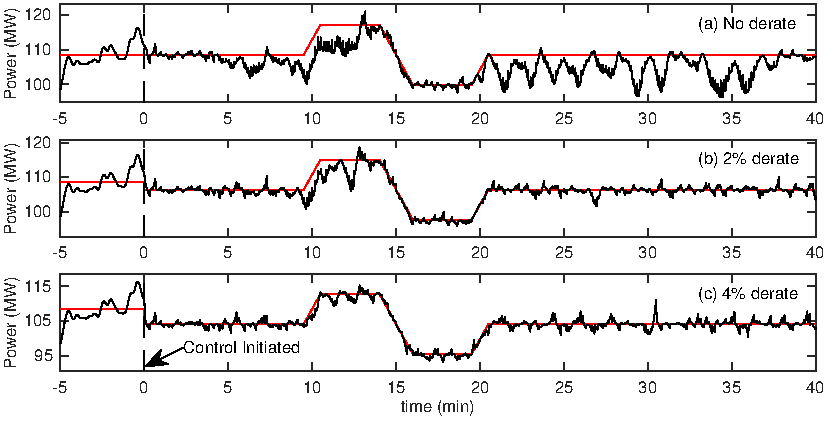
\includegraphics[width=\textwidth]{./fig/Pfarm.pdf}
\caption{Simulated total farm power from controlled LES (black) and reference signal (red) versus time for (a) no derate, (b) 2\% derate, and (c) 4\% derate cases with inflow condition 1. Control is started at t = 0 (denoted by vertical black dashed line), and the pre-control reference signal shows the five-minute pre-control average wind farm power production. Since the magnitude of the reference signal is different in each panel, the bounds of the ordinate are scaled to $P(t) \in [0.95 \min_{0 \le t \le T} P_\text{ref}(t), 1.05\max_{0 \le t \le T}  P_\text{ref}(t)]$.}
\label{fig:Pfarm}
\end{center}
\end{figure}

The power reference signal, shown in red in Figure~\ref{fig:Pfarm}, is specified as 
\begin{equation}
P_\text{ref}(t) = [1-\alpha + r(t) ]P_\text{base}.
\end{equation}
We define the baseline power $P_\text{base}$ as the five-minute average of the power output prior to the initiation of the control. Averaging over five-minute windows was found to provide reasonable averages; for an LES with a constant $C_T' = 1.33$ the root-mean-square of the total power output after averaging over five-minute windows is less than 2.5\% of the mean power output over a 45-minute period. The time-varying change in power setpoint $r(t)$ varies by $\pm 0.08$ and is meant to be representative of secondary frequency regulation signals used by grid operators~\cite{PJMm12}. The parameter $\alpha$ is the reduction in the power setpoints to compensate for the need to track increases in power demand. It is also a measure of the fraction of revenue lost for the supply of bulk power. We consider three different cases $\alpha = 0$, 0.02, and 0.04, which are referred to as derate cases because they correspond to derating the total power output by 0, 2, and 4\% for a given condition. These derates are not imposed by an \textit{a priori} reduction in the local thrust coefficient; instead, the controller imposes the derates by dynamically responding to the power reference signal at the initiation of the control. Each derate case is tested with three inflow initial conditions generated by separate atmospheric boundary layer simulations, resulting in nine total simulations of the control approach in LES.

Table~\ref{tab:rmse} compares the controller performance for the three derate cases under all three inflow conditions. For each inflow condition the baseline five-minute pre-control average power $P_\text{base}$ is provided. The error between the controlled LES wind farm power $P(t)$ and the reference signal $P_\text{ref}(t)$ is reported as the root mean square error 
\begin{equation}
\text{RMSE} = \left(\frac{1}{T} \int_0^T [P(t) - P_\text{ref}(t)]^2 \, dt\,\right)^{1/2}
\end{equation}
 in MW. To compare the performance between different inflow conditions, the RMSE normalized by the baseline power $\text{NRMSE} = \text{RMSE}/P_\text{base}$ is also provided. These results demonstrate that the RMSE decreases with increasing derate, indicating improved performance. Performance can also vary substantially depending on the inflow conditions, but this sensitivity decreases with increasing derate. 
 
\begin{table}
\caption{Comparison of controller performance for three derate cases and three inflow conditions. For each inflow condition the table reports the pre-control five-minute average power $\text{P}_\text{base}$. The error between the controlled LES wind farm power and the reference signal is reported as both the root mean square error (RMSE) in MW and normalized root mean square error (NRMSE) in \% relative to $\text{P}_\text{base}$ in MW.}
\label{tab:rmse}
\centering
\small
\begin{tabular}{c c c c c c c c}
\toprule
Inflow & & \multicolumn{2}{c}{No Derate} & \multicolumn{2}{c}{2\% Derate} & \multicolumn{2}{c}{4\% Derate} \\
Conditions & $P_{\text{base}}$  & RMSE  & NRMSE & RMSE & NRMSE & RMSE & NRMSE  \\
\midrule
1 & 108.6 & 4.30 & 3.96 & 1.63 & 1.50 & 1.07 & 0.98 \\
2 & 96.6 & 1.68 & 1.74 & 0.89 & 0.93 & 0.90 & 0.93 \\
3 & 99.2 & 1.05 & 1.05 & 0.90 & 0.90 & 0.89 & 0.90 \\
\midrule
Mean & & 2.34 & 2.25 & 1.14 & 1.11 & 0.95 & 0.94 \\
\bottomrule
\end{tabular}
\end{table}

Figure~\ref{fig:Pfarm} further illustrates the improved performance of the controller with increasing derate by comparing the total farm power from controlled LES for each case to the reference signal for the first inflow condition. This inflow case has the highest RMSE for all derate cases and thus illustrates the worst performance of the controller for each derate case. For the least successful simulation, the no derate case in Figure~\ref{fig:Pfarm}(a), the control has difficulty following the reference signal. For the 2\% derate case in Figure~\ref{fig:Pfarm}(b) the wind farm power generally follows the reference signal, except when the reference signal requires a large increase in power. For the 4\% derate case shown in Figure~\ref{fig:Pfarm}(c) the total farm power closely follows the reference signal with fluctuations about the reference. Interestingly, the mean power production during minutes 20--40 in the no derate case is lower than the other cases. This may be because the controller has extracted more kinetic energy from the flow field to try to meet the reference signal during the preceding 20 minutes and therefore cannot increase the power level further. Furthermore, the fluctuations during the controlled period are noticeably smaller than the pre-control fluctuations with constant $C_T'$. In other words, the control also damps the natural turbulent fluctuations in power output, which may also be beneficial for system operations.


These results demonstrate the importance of derating the power production in order to provide secondary frequency regulation. Since the power production will naturally fluctuate around an average production level, controlling power at the average may not be possible. For example, the controller is unable to maintain the baseline power during the last half of the control period in the no derate case shown in Figure~\ref{fig:Pfarm}(a). During periods where the reference signal is larger than the available energy from the inflow conditions the control will fail to track the power reference signal. This could also explain the failure to track the signal during the up-ramps in Figure~\ref{fig:Pfarm}(a)--(b), 

The importance of including aerodynamic interactions in the control strategy is highlighted by Figure~\ref{fig:Ctp}, which shows representative control trajectories in each row for inflow condition 3 with no initial derate. In particular, these results show that the control signal for the last row of farm, which does not influence the power output of upstream turbines, operates differently than the other rows. Furthermore, during the few minutes preceding the up-ramp of the reference signal, the thrust coefficients of the first six rows decline in order to move power generation from the first row to downstream rows, as shown in Figure~\ref{fig:P_contribution}. This movement towards a different operating state may allow the farm to extract additional power over a short period (10--15 minutes) by the slow ramping of the thrust coefficients. 

\begin{figure}[h]
\begin{center}
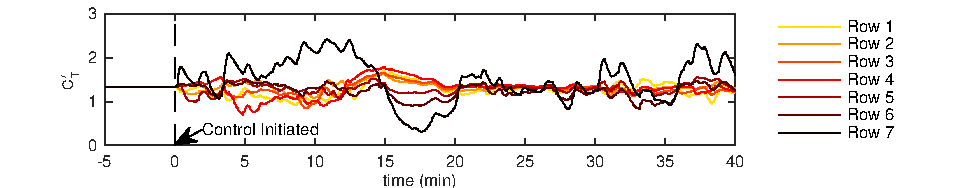
\includegraphics[width=\textwidth]{./fig/Ctp.pdf}
\caption{Control trajectories $\text{C}'_\text{T}$ of each row for inflow condition 3 and no initial derate.}
\label{fig:Ctp}
\end{center}
\end{figure}

\begin{figure}[b]
\begin{center}
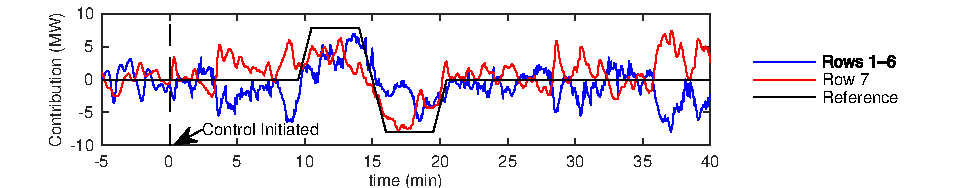
\includegraphics[width=\textwidth]{./fig/Pcont.pdf}
\caption{Contribution of first six rows and last row to the regulation for inflow condition 3 with no initial derate. The contribution is computed by subtracting the pre-control average power production for each collection of rows. The pre-control average power production for the entire farm is subtracted from the reference shown.}
\label{fig:P_contribution}
\end{center}
\end{figure}

By leveraging these aerodynamic effects, the proposed control strategy has demonstrated the potential to reduce the setpoint reduction used in previous work~\cite{Aho2013a, Aho2014a, Jeong2014a}, where the power production is derated by an amount equal to the maximum up-regulation of the signal. The consistent success of the 4\% derate case, indicates that for the test system and initial operating conditions used (LES with the actuator disk model) the derate can be 50\% of that normally employed in single turbine based control strategies. However, the required derate most likely depends on the maximum duration of the required up-regulation, the size of the wind farm, the wind farm spacing and configuration, and the thrust and power coefficient curves of the wind turbines, among other factors. Understanding these effects as well as others affection implementation are a direction for future work.

The reduced derate required to provide this power tracking service has large potential economic consequences for wind operators. Previous studies have indicated that the trade-off between payments from bulk power supply and participation in frequency regulation markets are important for the viability of wind farms participating in frequency regulation. Within the context of previous work, where wind farms were derated by an amount equal to the maximum up-regulation of the signal, the economic viability of wind farm secondary frequency regulation was of some debate~\cite{Kirby2010a, Rose2014a}. Reducing the required derate increases steady-state operating power generation, thereby allowing wind farm operators to provide a higher level of bulk power and still participate in frequency regulation markets; i.e. it reduces the cost burden of providing frequency regulation and may lead to increases in revenue due to the ability to provide this new service.

\section{Grid operator qualification tests}
\label{sec:rhc-pjm}
In this section, we evaluate the control approach described above with regulation test signals from PJM, an independent system operator (ISO) in the United States Eastern Interconnection~\cite{PJMm11, PJMm12}. PJM has two types of secondary frequency regulation signals that are based on the Area Control Error (ACE) signal, a combined measure of the power imbalance and deviation of the frequency from its nominal operating value. The ``RegA'' signal is a low pass filter of the ACE that is generally followed using traditional regulating resources, such as fossil fuel plants. The ``RegD'' signal is a high pass filter of the ACE that can be followed by more quickly responding resources, such as energy storage devices. We evaluate the performance of the controller using PJM's performance evaluation criteria~\cite{PJMm11, PJMm12} to determine whether the controlled wind farm system can meet PJM's threshold for qualification in these two regulation markets. These computations also allow us to evaluate whether wind farms with this control strategy are better suited to provide traditional or fast-acting regulation.

In order to participate in PJM's regulation market, power plants must pass the Regulation Qualification Tests for the particular regulation signal being supplied. These tests are carried out over a 40-minute period, and the tracking capability is quantified using a composite performance score, which is the weighted sum of accuracy, delay, and precision scores~\cite{PJMm11,PJMm12}. The accuracy score measures the ability of the signal to respond to a change in the ISO regulation signal. The delay score measures the delay in the plant's response to the regulation signal. The precision score measures the difference between the requested power and the plant's power output. A minimum composite score of 75\% is needed to qualify to participate in each of the two regulation services. Once qualified for a particular service, a plant is continuously evaluated; if its average score over the last 100 hours drops below 40\%, then the plant is disqualified from providing the service and must retake the initial performance tests to requalify. 

The performance of the controlled wind farms is evaluated using PJM's published RegA and RegD test signals as well as historical RegA and RegD signals from three hours in 2015~\cite{PJMm11,PJMm12, PJM2018a}. For each regulation signal, we use three different initial conditions for the wind farm and two levels of power derate. As in the previous section, the reference signal for each test is defined as $P_\text{ref}(t) = [1 - \alpha + 0.08r(t)]P_\text{base}$, where $P_\text{base}$ is the 5-minute average power prior to initiation of the control, $\alpha$ is the derate amount, and $r(t) \in [-1,1]$ is the regulation signal from the ISO. 

The combination of test signals and initial conditions lead to 48 unique test cases, each of which is given a unique identifier that is a combination of identifiers for each of the variable types shown in Table~\ref{tab:cases}. ``Signal'' refers to the regulation signal type (RegA or RegD), ``Derate'' refers the to derate amount (4 or 6\%), ``Initial condition'' refers to the initial condition of the controlled plant simulation, and ``Period'' refers to the regulation signal period, which is either the PJM test signals or one of the selected hours in 2015. For example, the test case ``RegA.D4.IC1.TS'' refers to the case with the RegA test signal, 4\% derate, and the first initial condition. 
%
\begin{center}
\begin{table}[t]
\caption{\label{tab:cases} Test case identifiers describing the signal type, derate amount, initial condition of the wind farm, and regulation signal period. For example, the test case ``RegD.D6.IC1.H2' refers to the case with the second RegD historical signal, 6\% derate, and the first initial condition.}
\centering
\begin{tabular}{@{}*{7}{l}}
\hline
Identifier & Type & Description\\
\hline
RegA & Signal & Traditional RegA regulation signal\\
RegD & Signal & Fast-responding RegD regulation signal\\
D4 & Derate & Power setpoint is reduced by 4\% of $P_\text{base}$\\
D6 & Derate & Power setpoint is reduced by 6\% of $P_\text{base}$\\
IC1 & Initial condition & Initial condition 1\\
IC2 & Initial condition & Initial condition 2\\
IC3 & Initial condition & Initial condition 3\\
TS & Period & PJM test signals\\
H1 & Period & PJM historical hour 1\\
H2 & Period & PJM historical hour 2\\
H3 & Period & PJM historical hour 3\\
\hline
\end{tabular}
\end{table}
\end{center}

\subsection{Historical PJM regulation signals}
\label{subsec:rhc-pjm-hist}
The number of historical hours used to test the controlled wind farm is constrained by the computational cost of running the model wind farm LES. As a result, it is impractical to select enough hours to sample the entire range of possible regulation signals provided by PJM. To prevent systematic bias, the three hours were selected without considering the characteristics of the regulation signals during those periods. 


\begin{figure}[t]
\begin{center}
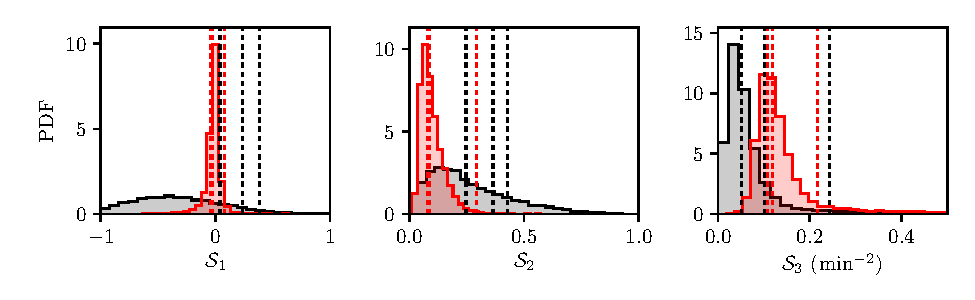
\includegraphics[width=\textwidth]{./fig/f4.pdf}
\end{center}
\caption{\label{fig:pdfs} Probability density functions of $\mathcal{S}_1$--$\mathcal{S}_3$ defined in Eq.~\eqref{eq:stats} for RegA (black) and RegD (red) during 2015. The three selected historical hours are shown in the PDFs as vertical dashed lines.}
\end{figure}

In order to evaluate whether the selected signals are representative cases, we compare them to the range of all possible regulation signals provided by PJM in 2015 using three statistics
\begin{equation}
\label{eq:stats}
\mathcal{S}_1 = \frac{1}{T}\int_0^T r(t) \, dt \qquad \mathcal{S}_2 = \frac{1}{T}\int_0^T r^2(t) \, dt - \mathcal{S}_1^2  \qquad \mathcal{S}_3 = \frac{1}{T}\int_0^T \left(\frac{dr}{dt}\right)^2 \, dt ,
\end{equation}
where $r(t)$ is the regulation signal, $T = 60$ min, $\mathcal{S}_1$ is the mean of $r(t)$, $\mathcal{S}_2$ is the variance of $r(t)$, and $\mathcal{S}_3$ is the variance of $\frac{dr}{dt}$. For each of these statistical measures, the probability density function (PDF) is calculated using all possible hourly signals provided by PJM in 2015 and is shown in Figure~\ref{fig:pdfs}. These PDFs demonstrate the differences between the RegA and RegD signals. The RegA signals have a larger mean and variance than the RegD signals, but the variance of $\frac{dr}{dt}$ is smaller. The values of these statistics for the three selected hours is compared to the PDFs over the entire year in Figure~\ref{fig:pdfs}. These figures show that the selected historical signals represent a reasonable cross section of the possible PJM regulation signals. The only exception, the high percentile ranking in $\mathcal{S}_1$ of the RegA signals, represents a more difficult test for the controlled wind farm because more energy is requested than the average.


\subsection{Wind farm initial conditions}
\label{subsec:rhc-pjm-ic}
We set the initial conditions of the controlled wind farm simulations to correspond to uncontrolled simulations with a local thrust coefficient of $C_{T,\text{ref}}'=1.33$, as previously discussed. The inflow characteristics for the three initial conditions of interest are provided in Table~\ref{tab:params}. The inflow velocities of the initial conditions have a mean $\overline{u} \approx 9.5$ m/s and a standard deviation $\sigma_u \approx 1$ m/s as measured at the first row of turbines during the $T_0 = 5$ min prior to initiation of the control
\begin{align}
\overline{u} &= \frac{4 + C_{T,\text{ref}}'}{4}\frac{1}{T_0 M} \int_{-T_0}^0 \sum_{m=1}^M u_{1m}(t) \, dt \\
\sigma_u &= \frac{4 + C_{T,\text{ref}}'}{4} \left[\frac{1}{T_0M} \int_{-T_0}^0\sum_{m=1}^M \left(u_{1m}(t) - \overline{u}\right)^2 \, dt \right]^{1/2}.
\end{align}
The turbulence intensity as measured at the center of each of the turbine rotors is approximately 13\%, which corresponds to low to medium IEC turbulence levels~\cite{IEC2005a}. The simulations assume region 2 operation~\cite{Johnson2006a} with idealized aerodynamic characteristics of $C_P' = C_T'$. In order to avoid any significant interaction with the rated regime, we presume wind turbines with a rated wind speed of at least 12m/s, which corresponds to the 99th percentile of the LES velocity field.

The required parameters of the static and dynamic wake models, inlet velocity $U_\infty$ and wake expansion coefficients $k_n$, are also calculated for each initial condition using measurements from the $T_0 = 5$ min prior to initialization of the control. The inlet velocity is set using the relationship $U_\infty =\frac{1}{4}(4 + C_{T,\text{ref}}')T^{-1}\int_{-T_0}^0 u_1(t) \, dt$, and the wake expansion coefficients are found using a least squares fit between the measured power and the power predicted by the static model. Note that the inlet velocity for the model is defined using the average power and therefore  the average inflow velocity is not equal to the inlet velocity for the models $\overline{u} \ne U_\infty$. The resulting parameters are also shown in Table~\ref{tab:params}.
%
\begin{center}
\begin{table}[h!]
\caption{\label{tab:params} Characteristics of the three wind farm initial conditions, including mean inlet velocity $\overline{u}$, standard deviation of inlet velocity $\sigma_u$, and turbulence intensity TI. The corresponding wake model inlet velocity $U_\infty$ and wake expansion coefficients $k_n$ are also shown.}
\centering
\begin{tabular}{@{}*{12}{l}}
\hline
Initial & $\overline{u}$ & $\sigma_u$& TI & $U_\infty$& $k_1$ & $k_2$ & $k_3$ & $k_4$ & $k_5$ & $k_6$ & $k_7$\\
condition & m/s & m/s & \% &  m/s & - & - & - & - & - & - & - \\
\hline
1 & 9.53 & 1.12 & 13.6 & 9.65 & 0.028 & 0.049 & 0.041 & 0.047 & 0.053 & 0.054 & 0.054 \\
2 & 9.22 & 0.97 & 13.3 & 9.32 & 0.026 & 0.046 & 0.043 & 0.047 & 0.054 & 0.052 & 0.052 \\
3 & 9.56 & 0.93 & 12.5 & 9.64 & 0.026 & 0.040 & 0.040 & 0.037 & 0.044 & 0.041 & 0.041 \\
\hline
\end{tabular}
\end{table}
\end{center}

\subsection{Results and discussion}
\label{subsec:rhc-pjm-results}
The time evolution of the total controlled LES wind farm power is compared to the reference signals for initial condition 3 and a 4\% derate in Figure~\ref{fig:pfarm4}, which shows all regulation signals (RegA or RegD) and regulation period combinations. The controlled wind farm power production is also compared to the uncontrolled case, where the wind farm is kept at the constant pre-control thrust coefficient. These results demonstrate the good overall tracking performance of the controlled wind farm, except for a few specific periods of under-performance. Furthermore, the results demonstrate that the dynamic-model based receding horizon control method is able to reduce the natural turbulent fluctuations in the wind farm power production. Indeed, the root-mean-square (RMS) of the controlled wind farm power production about the reference signal is 1.06 MW, which is almost a quarter of the 3.93 MW RMS of uncontrolled power production about the baseline power. 

\begin{figure}[t]
\begin{center}
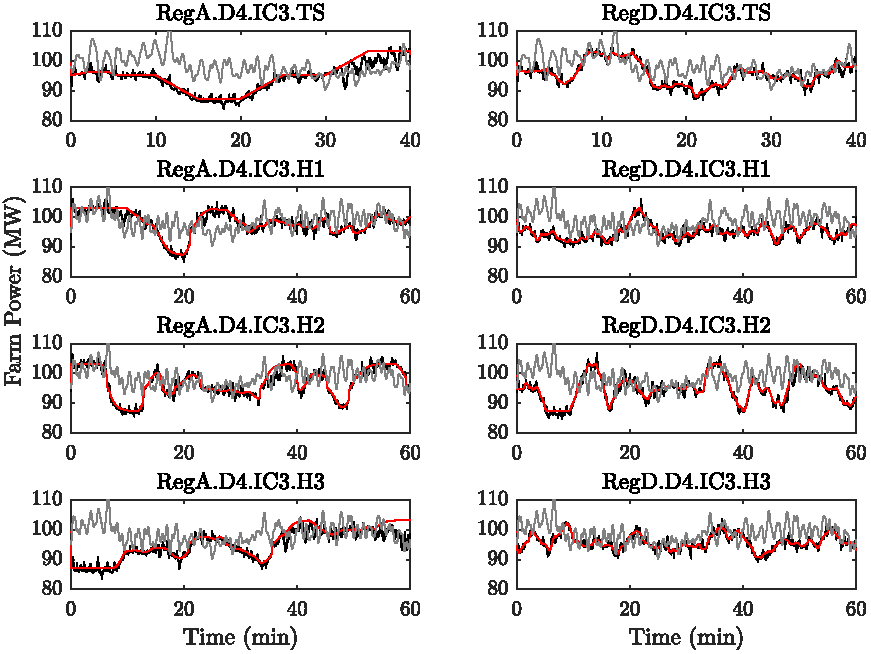
\includegraphics[width=\textwidth]{./fig/f8.pdf}
\end{center}
\caption{\label{fig:pfarm4}Power tracking performance of dynamic-model controlled wind farms comparing simulated farm power from a controlled LES wind farm model (------), an uncontrolled LES wind farm model ({\color{gray}------}), and power reference signals ({\color{red}------}) for 4\% derates and initial condition 3.}
\end{figure}

Quantitative measures of the performance of each regulation signal type (RegA or RegD) for derate values of 4\% and 6\% are shown in terms of PJM's performance scores in Figure~\ref{fig:boxplots}. The controlled wind farm performs better for the RegD signals, meeting the composite score threshold for qualification of 75\% in all cases. The performance of the controlled farm in tracking the RegA signals is also satisfactory for PJM participation, but the controlled farm would not have qualified in all tests. These lower composite scores may be explained by the large values in $\mathcal{S}_1$, which represent the total energy requested in the signals, compared to other PJM signals. However, in cases where the controlled wind farm had poor performance for the RegA signal with 4\% derate, increasing the derate to 6\% markedly improved the overall performance.

\begin{figure}[h]
\begin{center}
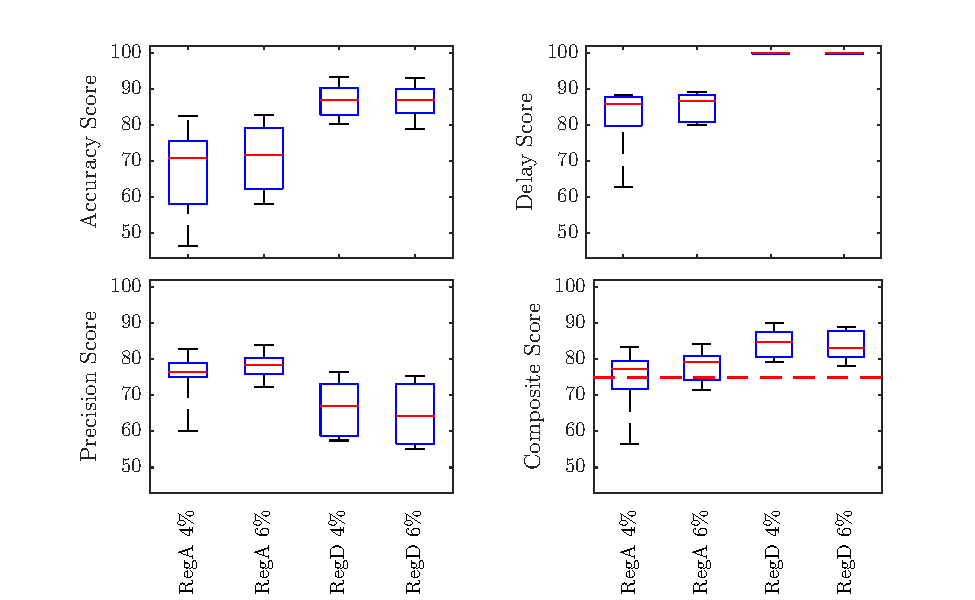
\includegraphics[width=\textwidth]{./fig/f9.pdf}
\end{center}
\caption{\label{fig:boxplots}Boxplots of PJM performance scores for dynamic-model controlled wind farm for all regulation signal types (RegA or RegD) with derate values of 4\% and 6\%. The qualification threshold of 75\% for the composite score ({\color{red}--- --- ---}) is shown in the lower right panel. The average controlled system performance exceeds the 75\% for both signal types, but only the RegD cases pass all of the time.}
\end{figure}

The results shown in Figures~\ref{fig:boxplots}--\ref{fig:reg_a_4d} provide important insights into the possible strengths and limitations of the proposed approach to wind farm control for frequency regulation. These results suggest that wind farms may be well suited to act as a quickly responding resource for grid regulation services. For example, the consistent passing of the composite performance score for the RegD signals indicates that dynamic-model controlled wind farms are able to provide this service reliably. 

The power tracking results in Figure~\ref{fig:pfarm4} demonstrate that the controller is able to track the up-regulation portions of the RegA signals at the beginning of the control period, such as during the first 5--10 minutes of the first two historical signals. In several cases the controlled LES wind farm is able to produce more power than the uncontrolled case, such as after minute 20 of the ``RegA.D4.IC3.H1'' and ``RegD.D4.IC3.H1'' simulations. However, when up-regulation is requested for prolonged periods or towards the end of the control interval, such as the last 10 minutes of the ``RegA.D4.IC3.TS'' and ``RegA.D4.IC3.H3'' cases, the controller does not perform as well. A possible explanation is that the available energy in the wind is slowly changing as the atmospheric boundary layer evolves, as demonstrated by the declining power production of the uncontrolled simulations during these time periods. Since estimates of available energy are readily available over short time horizons, more frequent market clearing may allow wind farms to more effectively provide regulation. Ultimately, future work is needed to determine whether this is a fundamental limitation of the wind farm dynamics or the control strategy and whether additional sensing or forecasting data can overcome these issues.

\section{Comparison to static wake model control}
\label{sec:rhc-static}
In this section we consider the effect of reducing the control design and wake model complexity. In particular, we evaluate the importance of explicitly modeling the dynamics of wake advection by comparing the performance of the dynamic-model approach to a similar static-model approach; i.e. we replace the dynamic wake model with the Jensen model~\cite{Katic1986a}. The standard Jensen model assumes each turbine generates a wake region that expands radially at a linear rate $k$ with increasing downstream distance from the turbine. This leads to following definition of the wake diameter 
\begin{equation}
\label{eq:dw}
D_w(x) = D + 2kx,
\end{equation} 
where $x$ is the streamwise distance from the turbine rotor plane. 

Conservation of mass leads to the following velocity deficit in the wake of the $m$-th turbine in the $n$-th row
\begin{equation}
\label{eq:jens-delta}
\delta u_{nm}(x)  = \frac{2 U_\infty a_{nm}}{\left[D_w(x-s_n)/D\right]^2},
\end{equation}
where $a_{nm}$ is the induction factor and $U_\infty$ is the velocity upstream of the wind farm. This representation yields top-hat profiles of velocity deficits in each cross-stream plane. The velocity field experienced by the each turbine is found by superimposing the squared velocity deficits
\begin{align}
\label{eq:jens-uinfty}
u_{\infty nm} &= U_\infty -\sqrt{ \sum_{(j,k) \in \mathcal{S}_{nm}} \delta u_{jk}^2(s_n-s_j)},
\end{align}
where $\mathcal{S}_{nm}$ is defined as the set of turbines whose wakes lie within the swept area of the turbine rotor of the $m$-th turbine in row $n$. The definition of these sets means that Eq.~\eqref{eq:jens-uinfty} reduces to $u_{\infty1m} = U_\infty$ for the first row of turbines. The power production of each turbine is subsequently found using 
\begin{equation}
\label{eq:Pjens}
\hat{P}_{nm} = \frac{1}{2}\rho\frac{\pi D^2}{4} C_{Pnm} u_{\infty nm}^3,
\end{equation}
where $C_{P nm}$ is the power coefficient of the turbine in row $n$ and column $m$.

To make the Jensen model used here comparable to the dynamic model discussed in Section~\ref{sec:dynwake-1d}, we make the following modifications to the standard Jensen model. First, we consider each row of turbines collectively, which means that each modeled value is homogeneous in the spanwise direction and we neglect the spanwise merging of wakes. To reflect this modification, the column index $m$ used in the Eqs.~\eqref{eq:jens-delta}--\eqref{eq:jens-uinfty} is dropped in subsequent equations. Second, to account for entrance effects in the farm and compensate for the neglected spanwise wake interactions, we allow each wind turbine row to have a separate wake expansion rate $k_n$. 

Furthermore, we express the turbine power production using the local thrust coefficient $C_{Tn}'$ and modeled velocity at the turbine rotor $\hat{u}_n$. From momentum theory, we know that
\begin{equation}
\label{eq:relationships}
a_n = \frac{C_{Tn}'}{4+C_{Tn}'}, \qquad \hat{u}_n = (1-a_n) u_{\infty n}, \quad \text{and}  \qquad  C_{Tn}' = C_{Pn}' = \frac{C_{Tn}}{(1-a_n)^2}.
\end{equation}
Replacing  the induction factor $a_n$ in Eq.~\eqref{eq:jens-delta},  the modeled upstream velocity $u_{\infty n}$ in Eq.~\eqref{eq:jens-uinfty}, and the power power coefficient $C_{Pn}$ in Eq.~\eqref{eq:Pjens} with these equations, the power production can be rewritten as 
\begin{equation}
\label{eq:power-hat}
\hat{P}_{n} = M\frac{1}{2}\rho\frac{\pi D^2}{4} C_{Tn}' \hat{u}_n^3.
\end{equation}

The static wake model used in this work is the Jensen model with the modifications described above. In order to use this static wake model in a model-based controller for the farm power production, the model must be augmented to account for time-varying changes in the local thrust coefficient $C_{Tn}'(t)$. Including time dependency in the thrust coefficient and replacing the induction factor in Eq.~\eqref{eq:jens-delta} with the expression in Eq.~\eqref{eq:relationships} gives the following expression for the velocity deficit for the $n$-th turbine 
\begin{equation}
\label{eq:static1}
\delta u_n(x,t)  = \frac{C_{Tn}'(t)}{4 + C_{Tn}'(t)}\frac{2 U_\infty}{\left[1 + 2k_n (x - s_n)/D\right]^2}.
\end{equation}
With this approach, thrust coefficient changes instantaneously affect the velocity deficit everywhere; i.e., the wakes implicitly have an infinitely fast advection speed. Finally, the velocity at the turbines of the $n$-th row can be found by explicitly writing out the set of upstream turbines in Eq.~\eqref{eq:jens-uinfty} affecting the velocity at the $n$-th turbine and using the equation for the rotor-averaged velocity in Eq.~\eqref{eq:relationships}
\begin{equation}
\label{eq:static2}
\hat{u}_n(t) = \left(1- \frac{C_{Tn}'(t)}{4 + C_{Tn}'(t)}\right)\left( U_\infty - \sqrt{  \sum_{m=1}^{n-1} \delta u_m^2(s_n-s_m) } \, \right).
\end{equation}
Eqs.~\eqref{eq:static1} and~\eqref{eq:static2} are therefore the static wake model equations $\mathbf{W}_s(\mathbf{C}_{T}', \mathbf{q}_s) = \mathbf{0}$, where $\mathbf{q}_s = [\boldsymbol \delta \mathbf{u}, \mathbf{\hat{u}}]$ denote the model states and boldface indicates vectors. 

In order to make appropriate comparisons, the static-model controller solves an online optimization problem with feedback similar to that solved in the dynamic-model controller. As in the dynamic-model controller of Section~\ref{sec:rhc-control}, the static-model controller calculates the local thrust coefficient trajectories by repeatedly solving a minimization problem of the form
\begin{align}
\label{eq:minimize_J_static}
\underset{\mathbf{C_{T}'}, \mathbf{q}}{\text{minimize}} \qquad & \mathcal{J}(\mathbf{C_T'}, \mathbf{q} ) \\
\label{eq:constraint1_static}
\text{subject to} \qquad & \delta u_n(x,t)  = \frac{C_{Tn}'(t)}{4 + C_{Tn}'(t)}\frac{2 U_\infty}{\left[1 + 2k_n (x - s_n)/D\right]^2}\\
\label{eq:constraint2}
& \hat{u}_n(t) = \left(1- \frac{C_{Tn}'(t)}{4 + C_{Tn}'(t)}\right)\left( U_\infty - \sqrt{  \sum_{m=1}^{n-1} \delta u_m^2(s_n-s_m) } \, \right).
\end{align}
where the cost function is
\begin{equation}
\begin{split}
 \mathcal{J}(\mathbf{C_T'}, \mathbf{q} ) =& \frac{1}{\mathcal{P}^2}\left( \sum_{n=1}^N \hat{P}_n(t) - P_{\text{ref}}(t)\right)^2 + \eta \sum_{n=1}^N\left( C_{Tn}'(t) - C_{T, \text{ref}} \right)^2 \\
 &+ \gamma T^2 \sum_{n=1}^N\left( \frac{d C_{Tn}'}{dt}  \right)^2.
 \end{split}
\end{equation}
The constants $\mathcal{P}$, $\gamma$, and $\eta$ are the same as those used in the dynamic-model controller. Although both controllers solve an online optimization problem, the mechanics of the implementation are quite different. Since the equations for the static model have no dynamics, every instance in time is uncoupled. Therefore, the static-model controller can consider each point in time as a separate minimization problem, and the cost functionals can be written solely in terms of the current state. The dynamic-model controller in Section~\ref{sec:rhc-control}, on the other hand, accounts for the time-dependent advection of turbine wake.  Consistent with the distinction between the non-predictive and predictive nature of the static-model and dynamic-model controllers, the functionals for the static wake model are not integrated forward in time. In other words, the static wake model is not a receding horizon method because the modeled system does not include dynamics.

\subsection{Results and discussion}
\label{subsec:rhc-static-results}
The power tracking performance and control trajectories of the controlled wind farm, represented by the LES described in Section~\ref{subsec:methods-les-farm}, are shown in Figures~\ref{fig:reg_a_4d} and~\ref{fig:reg_d_4d}. The left and right panels of these figures show the performance of the static and dynamic-model controllers, respectively. Figure~\ref{fig:reg_a_4d} shows the response of the controlled farms to the RegA test signals, and Figure~\ref{fig:reg_d_4d} shows the response of the controllers to the RegD test signals. The dynamic-model control demonstrates good overall tracking performance, although it has some trouble tracking the reference signal during the last 5--10 minutes of the RegA.D4.IC1.TS and RegA.D4.IC3.TS cases. On the other hand, the static-model control demonstrates poor overall tracking performance, although it is able to track the signal for certain down regulation events, e.g. around minute 20 in all cases in Figure~\ref{fig:reg_a_4d}.

The static-model control method appears to switch between two distinct operating points, depending on the characteristics of the regulation signal. Down-regulation trajectories are often successfully tracked by increasing the thrust coefficient of the first row of turbines to values above \mbox{$C_T'=2$}. This change in operating conditions increases the magnitude of the velocity deficits throughout the farm, thereby reducing the overall wind speed throughout the farm and total power production. When there is a period of up-regulation approaching or the wind farm is slightly underproducing, the controller quickly reduces the upstream thrust coefficients and moves to the Betz-optimal thrust coefficient \mbox{$C_T'=2$} \cite{Goit2015a} for the last row. This operating point is likely the optimal power point for the Jensen model with constant wake expansion coefficients.

\clearpage 

\begin{figure}[h!]
\begin{center}
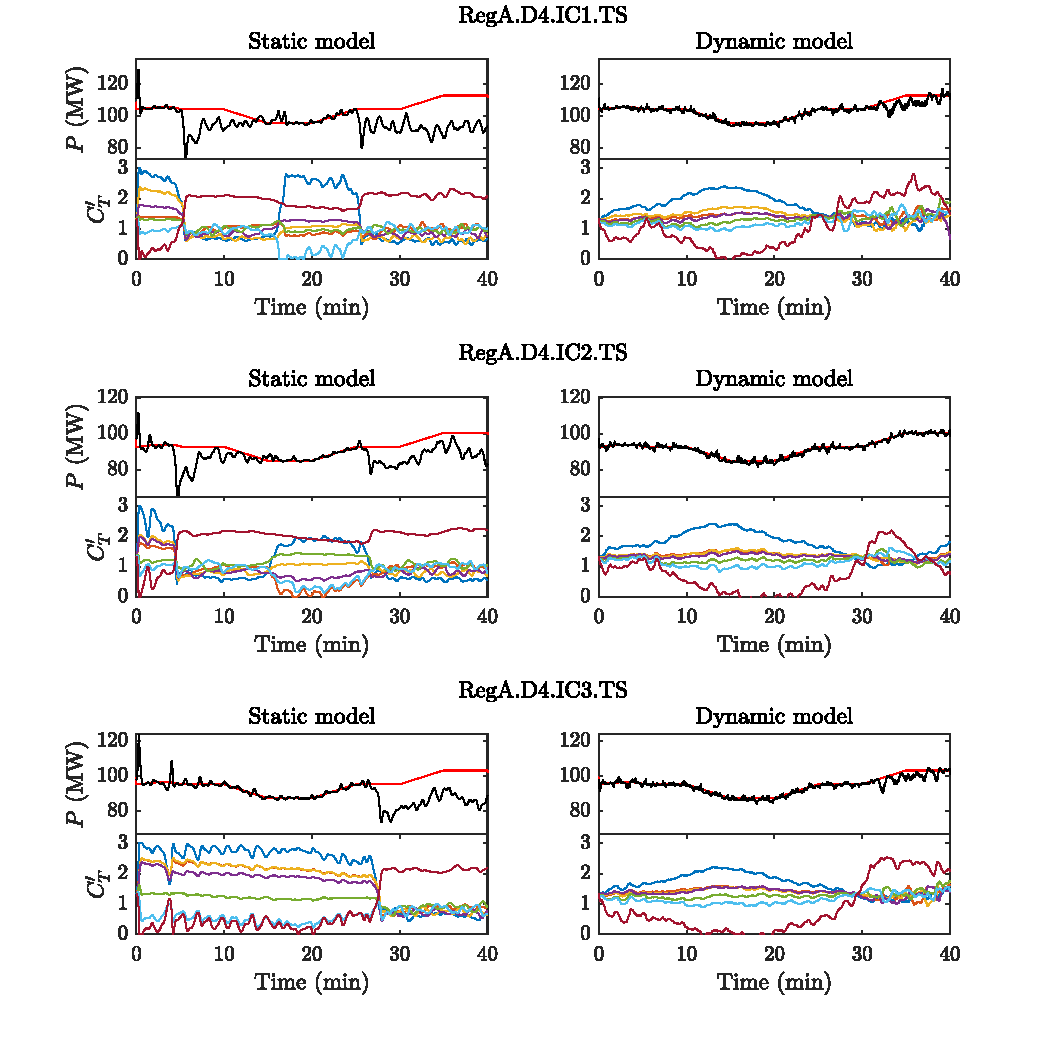
\includegraphics[width=\textwidth]{./fig/f5.pdf}
\end{center}
\caption{\label{fig:reg_a_4d} Comparison of static-model (left) and dynamic-model (right) control methods for RegA test signals with 4\% derates. All three initial conditions 1--3 are shown from top to bottom. The top panel in each row shows the controlled LES wind farm model power production (------) compared to the reference signal ({\color{red}------}). The bottom panel in each row shows the local thrust coefficients calculated by control methods by row: row  1 ({\color{co1}------}), row  2 ({\color{co2}------}), row  3 ({\color{co3}------}), row  4 ({\color{co4}------}), row  5 ({\color{co5}------}), row  6 ({\color{co6}------}), row  7 ({\color{co7}------}).}
\end{figure}

\begin{figure}[h!]
\begin{center}
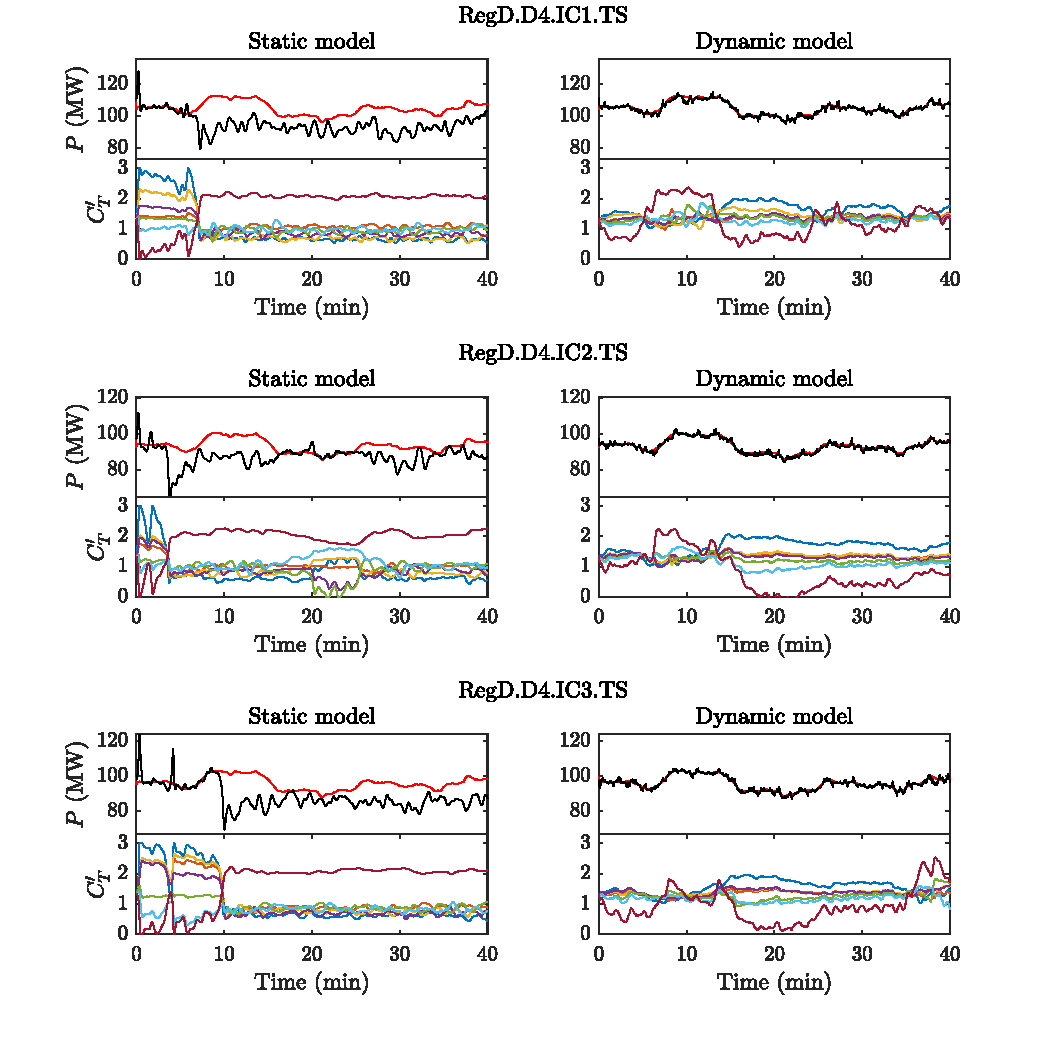
\includegraphics[width=\textwidth]{./fig/f6.pdf}
\end{center}
\caption{\label{fig:reg_d_4d} Comparison of static-model (left) and dynamic-model (right) control methods for RegD test signals with 4\% derates. All three initial conditions 1--3 are shown from top to bottom. The top panel in each row shows the controlled LES wind farm model power production (------) compared to the reference signal ({\color{red}------}). The bottom panel in each row shows the local thrust coefficients calculated by control methods by row: row  1 ({\color{co1}------}), row  2 ({\color{co2}------}), row  3 ({\color{co3}------}), row  4 ({\color{co4}------}), row  5 ({\color{co5}------}), row  6 ({\color{co6}------}), row  7 ({\color{co7}------}).}\end{figure}

\clearpage

\begin{figure}[b!]
\begin{center}
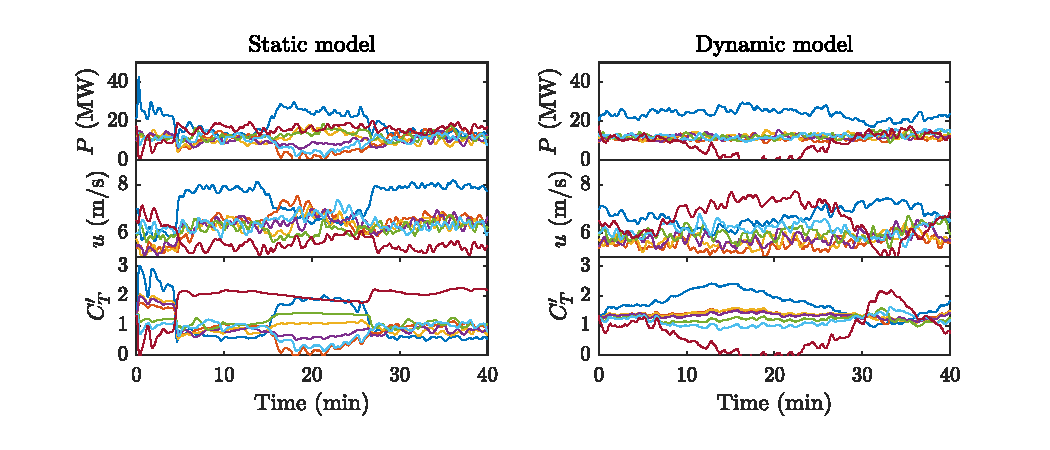
\includegraphics[width=\textwidth]{./fig/f7.pdf}
\end{center}
\caption{\label{fig:reg_a_4d-all} Comparison of static-model (left) and dynamic-model (right) control methods for RegA.D4.IC2.TS simulation case. Each panel shows the controlled LES wind farm model power production, rotor-averaged velocity, and thrust coefficients by row: row  1 ({\color{co1}------}), row  2 ({\color{co2}------}), row  3 ({\color{co3}------}), row  4 ({\color{co4}------}), row  5 ({\color{co5}------}), row  6 ({\color{co6}------}), row  7 ({\color{co7}------}).}\end{figure}

The performance of the static-model control provides an interesting demonstration of the importance of including time dependency in the wake model used in the type of model-based receding horizon control for frequency regulation described in this chapter. In an attempt to track the changing reference signal, the controller switches quickly between the two operating points discussed above. The static Jensen model erroneously models these transitions between operating points as an instantaneous change of the wake velocity deficit throughout the farm. In reality, the air around the turbine will slowly respond to a sudden change in the thrust coefficient and the reduced wake deficit must travel through the farm before the effects of changing upstream thrust coefficients on downstream power production and wind speeds are realized. Detailed trajectories of the power and rotor-averaged velocity of each row in Figure~\ref{fig:reg_a_4d-all}  show that the LES wind farm does not respond instantaneously to the change in operating point. Instead, power production slowly increases between minutes 5 and 15.

As a result of these modeling errors, the static-model controller produces large transient variations in power production when moving between operating points. When moving to the up-regulation operating point identified by the controller, the power production of the farm plunges. In some cases, the total power production slowly recovers to the desired setpoint. Furthermore, all of the static-model control cases in Figures~\ref{fig:reg_a_4d} and~\ref{fig:reg_d_4d} demonstrate significant overshoot in the power production during the first 30 seconds of the simulations as the thrust coefficients quickly move away from the pre-control level. 

The dynamic-model control uses strategies similar to those of the static-model controller, including increasing the thrust coefficient during down-regulation periods and moving toward a Jensen model optimal power point for up-regulation periods. However, by including the time-dependent effects of wake advection, the controller avoids large transient changes when changing between states. The underlying dynamic model can correctly predict the time-varying effect of changing upstream thrust coefficients on downstream power production.

\section{Closed-loop controller with EnKF state and parameter estimation}
\label{sec:rhc-enkf}
In this section we several improvements to the controller introduced in Section~\ref{sec:rhc-control} and implemented in Sections~\ref{subsec:rhc-pjm-hist} and~\ref{subsec:rhc-pjm-ic}. First, we implement the improved state and parameter estimation methods of Section~\ref{subsec:estimation-ensemble-wake}. Second, we eliminate the regulation terms of the cost functional and introduce an auxiliary control variable to keep the control actions within physically acceptable ranges. Finally, we implement a constrained Quasi-Newton optimization method to increase the speed of the control.

In this implementation, we use a cost functional that represents the power tracking problem by penalizing deviations from the reference power $P_\text{ref}(t)$
\begin{equation}
\mathcal{J} = \int_{t_0}^{t_0+T} \left( \sum_{n=1}^N \hat{P}_n(t) - P_\text{ref}(t) \right)^2 \, dt,
\end{equation}
where $t_0$ is the current time. Using this cost function, we solve the following minimization problem
\begin{align}
\label{eq:minimize_J_enkf}
\underset{\boldsymbol \varphi(t), \mathbf{q}(x,t)}{\text{minimize}} \qquad & \mathcal{J}(\mathbf{q}(x,t)) \\
\label{eq:constraint1_enkf}
\text{subject to} \qquad& \mathbf{W}(\mathbf{q}(x,t)) = \mathbf{0} \\
\label{eq:constraint2_enkf}
& \frac{dC_{Tn}'}{dt} = \frac{1}{\tau} \left[ \varphi_n(t) - C_{Tn}'(t)\right]\\
\label{eq:constraint3_enkf}
& 0 \le \varphi_n(t) \le 2.
\end{align}
where $\mathbf{q}(x,t) = [\boldsymbol \delta \mathbf{u}(x,t), \mathbf{\hat{u}}(t), \mathbf{C}_T'(t)]$, $\boldsymbol \varphi(t)$ are auxiliary control variables, and $\mathbf{W}(\mathbf{q}(x,t)) = \mathbf{0}$ represents the wake model discussed of Section~\ref{sec:dynwake-1d}. The auxiliary control variables $\boldsymbol \varphi(t)$, whose rate of change is unconstrained, are used to prevent high-frequency oscillations of the local thrust coefficient. By specifying $\mathbf{C}_T'(t)$ through a  first-order relaxation of $\boldsymbol \varphi(t)$ with a time constant $\tau$, the rate of change of $\mathbf{C}_T'(t)$ is implicitly limited. Furthermore, we select bounds on the control variables of $\varphi_n(t) \in [0, 2]$ to prevent the local thrust coefficient from becoming negative or exceeding the Betz limit of $C_T'=2$~\cite{Meyers2016a}. Minimization is performed using the limited-memory bound-constrained quasi-Newton method L-BFGS-B~\cite{Zhu1997a}. 

With the time horizon and advancement time parameters that are employed in this implementation, as well as the optimization method used, each minimization problem is solved in a fraction of the advancement time on a single processor. In this implementation, we choose a time horizon of $T = 10$ min, which is longer than the time it takes for the wind to travel across the seven-row wind farm considered here, and an advancement time of $T_A \approx 1$ s. This speed is accomplished by using the adjoint equations to compute the gradient, limiting the number of iterations of the minimization algorithm, and using the optimization solution over the previous time horizon as an initial guess for the next time horizon. As a result, this control algorithm can be implemented in real time.

The controlled wind farm is tested in twelve total simulations. We use derates of $\alpha = 0.04$ and 0.06. The signal $r(t)$ is taken from the PJM RegA and RegD test signals~\cite{PJMm11, PJMm12}.  Each derate and signal type combination is tested using all three ending states of the EnKF test cases in Section~\ref{subsec:estimation-ensemble-validation}.

The performance of the controlled wind farm is shown for all twelve simulations in Figure~\ref{fig:enkf-rhc}. Each panel shows the reference signal as described above, the controlled power output, and the uncontrolled power output if the pre-control thrust coefficient $C_{Tn}' = 1.33$ were continued from $t=0$ using the same wind farm state. The performance of the controlled wind farm under the first two initial conditions demonstrate good tracking performance for the the slowly-varying RegA signals as well as the fast-acting RegD signal. The rate-limiting of the control actuation filter results in noticeable fluctuations around the requested power reference signal and some overshoot at the beginning of the control period. However, the controlled farm power has noticeably smaller fluctuations than the turbulent fluctuations of the uncontrolled power. By reducing turbulent fluctuations, the wind farm behaves more like a conventional generator by providing more consistent power output to the grid.


\begin{figure}[h!]
\centering
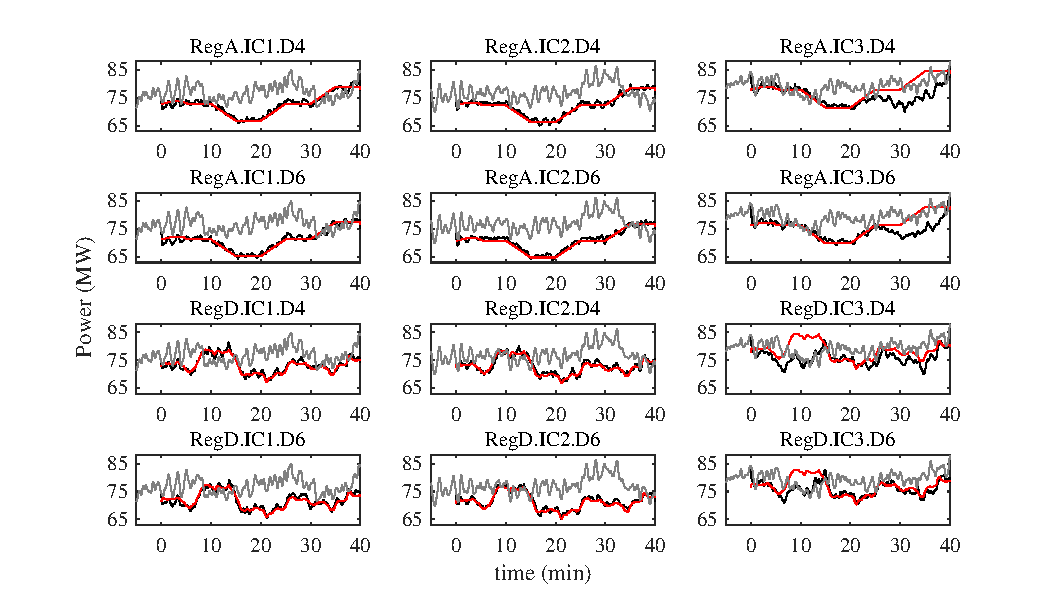
\includegraphics[width=\textwidth]{./fig/enkf-rhc.pdf}
\caption{Controlled wind farm power output (\full) compared to reference signal ({\color{red}\full}) and uncontrolled wind farm power output({\color{gray}\full}). All twelve simulations are shown and denoted by the signal type (RegA or RegD), the initial conditions (IC1--IC3), and derate (D4 for 4\% and D6 for 6\%).}
\label{fig:enkf-rhc}
\end{figure}
These simulations also demonstrate the importance of including a dynamic wake model into the model-based receding horizon control design. During some periods of the simulation---such as around the 10-minute mark of the RegD.IC1.D4 signal and the last 5 minutes of the RegA.IC2.D4 signal---the controlled wind farm was able to produce more power than the uncontrolled farm. Similar trends were seen in Sections~\ref{sec:rhc-control} and~\ref{sec:rhc-static}, where the controller is able to reduce the energy extraction of upstream turbines during periods with more available energy in the flow field, thereby providing increased power production potential for downstream rows. This mechanism would allow for increased production for a short duration by deferring upstream wind turbine energy extraction.

The relatively poor tracking performance of the third initial condition requires further investigation. Periods where the uncontrolled wind farm produces more power than the controlled farm are particularly hard to explain. In some cases, such as the under-production during the last twenty minutes of the RegA cases with the third initial condition, the uncontrolled farm produces more power than requested by the reference signal prior to the period. Therefore, the controlled wind farm probably has at least as much kinetic energy stored in its flow field as the uncontrolled case during this period. Determining the cause of this behavior is the focus of ongoing work.

On the other hand, the under-production around the 10 minute mark of the RegD.IC3.D4 and RegD.IC3.D6 signals in Figure~\ref{fig:enkf-rhc} is likely due to insufficient energy availability. The uncontrolled farm produces less power than requested by the reference signal, and the wind farm may be unable to accommodate the significant increased production requested by the grid operator. In other words, there simply may not be enough available kinetic energy in the flow field to provide the required level of power during this time period.

\section{Conclusions}
In this chapter, we showed that a wind farm using model-based receding horizon controller built around a dynamic wake model (see Section~\ref{sec:dynwake-1d}) can effectively provide secondary frequency regulation for the power grid. The controlled wind farm not only passes numerous qualification tests from PJM, a grid operator in the United States, but can provide secondary frequency regulation with smaller derates than single-turbine controllers. This has important implications for improving the profitability of wind farms providing secondary regulation. This derate reduction is accomplished by leveraging the dynamics of advection and wake dynamics through the wind farm, the controller can store kinetic energy in the flow field for a short period of time. Furthermore, we demonstrated that using a dynamic model is necessary to provide acceptable power tracking by comparing the control method to a similar controller built around the static Jensen model. Finally, we showed how the state and parameter estimation method of Section~\ref{subsec:estimation-ensemble-wake} can be incorporated allow continuous operation of the controller.